% Note that this file is not supposed to be wrapped in 'songs' environment.

\vfill%
\begin{figure}[!ht]%
  \centering%
  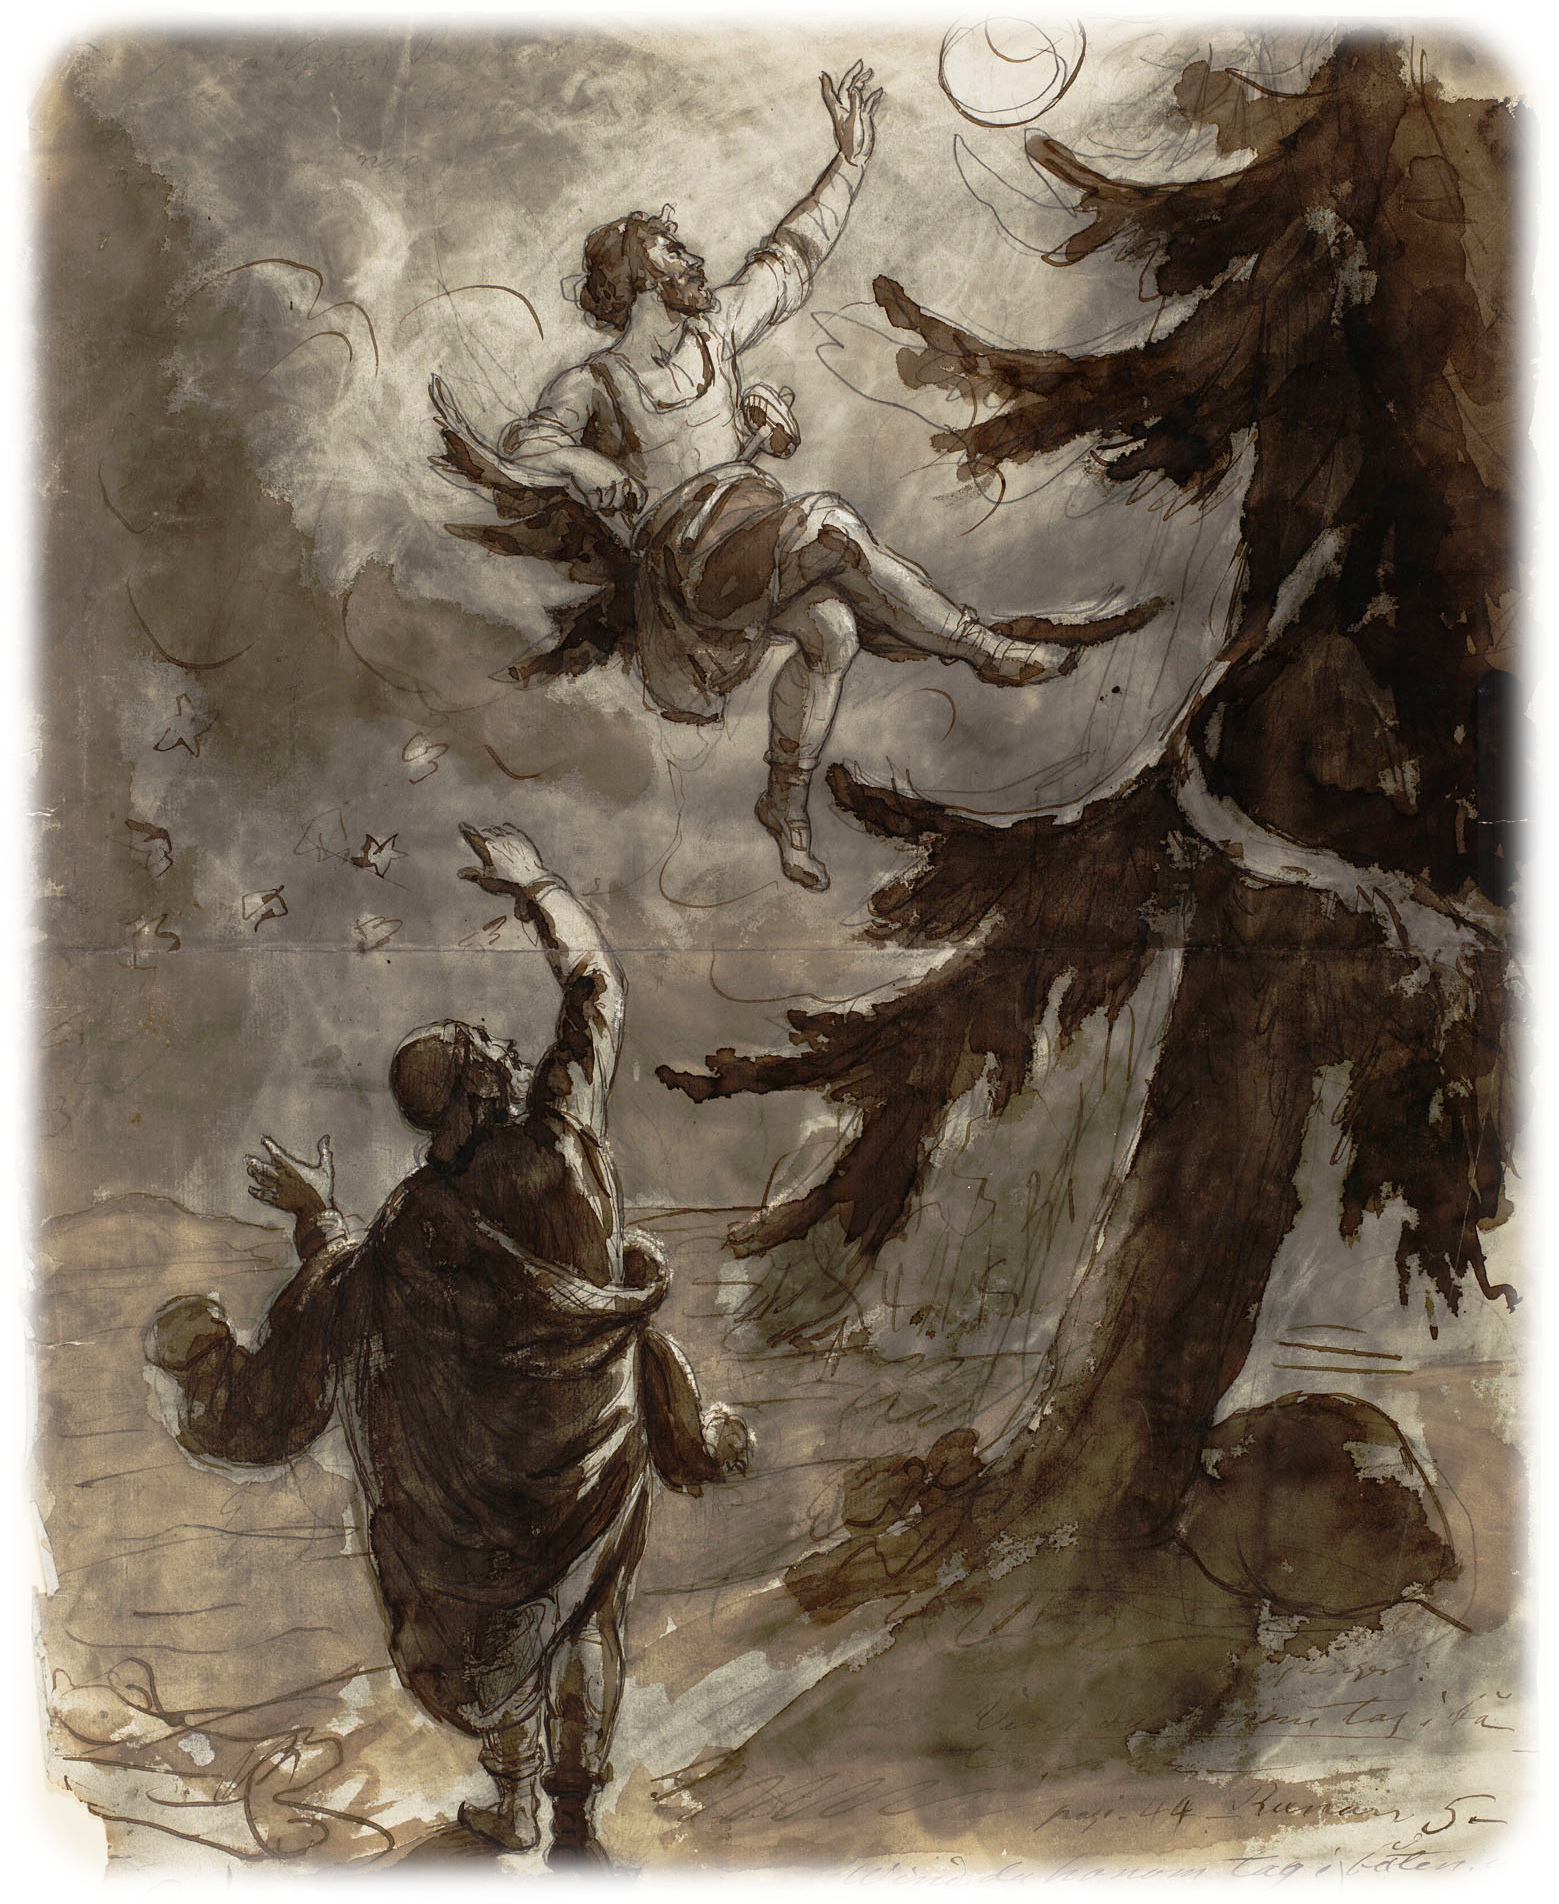
\includegraphics[width=0.82\textwidth]{Robert_Wilhelm_Ekman_-_Vainamoinen_laulaa_loitsuja_PD.jpg}%
  \caption{R. W. Ekman: Väinämöinen laulaa loitsuja}%
\end{figure}
\vfill%


\clearpage
\subsection{Luonnon nostatus}
  \paragraph{}
  \begin{large}\begin{center}\begin{em}
    Luontoani nostattelen\\
    haastattelen haltijata\\
    Nouse luontoni lovesta\\
    Syntyni syvästä maasta\\
    Syntyni syvästä maasta\\
    \vspace{1em}
    Maasta hauna haltijani\\
    Nouse niin kuin nousit ennen\\
    Minun nostatellessani\\
    \vspace{1em}
    Isoni luonto, emoni luonto\\
    Luonto valta vanhempani\\
    Oman luontoni lisäksi\\
    Nosta Ukon voima taivahasta\\
    Maasta maan Emoisen voima\\
    \vspace{1em}
    Tuekseni turvakseni väekseni voimakseni\\
    Tulkaa tarvittaessa, käykää kutsuttaessa\\
    Terveyttä tekemään rauhaa rakentamaan\\
    \vspace{1em}
  \end{em}\end{center}\end{large}

  \paragraph{}
  %\begin{em}
    Eräs kielemme vanhimmista sanoista on ``noita'', joka on alunperin tarkoittanut tietäjää eli
    shamaania. Kristillisellä aikakaudella noita sai kielteisen kaiun. Sitä ennen tietäjät
    olivat arvokas osa yhteisöä, jonka jäseniä he tukivat sairauksissa ja elämän murroskohdissa.
    \par
    Sekä loveen lankeaminen että haltioituminen ovat tietäjien tapoja saavuttaa taianomainen
    mielentila, jossa he saavat apua esivanhemmiltaan tai suojelushengiltä.
  %\end{em}

  \paragraph{Lovi} on yliluonnollinen paikka tai olotila, aukko arkitodellisuuden ja alisen
    maailman välillä. Aliseen maailmaan kuuluu vainajala taikka Tuonela, jossa esi-isät asustavat.
    Lovi sijaitsee joko maan tai veden alla --- ilmeisesti myös naisten hameen alla, sillä
    kansanrunojen mukaan sieltäkin löytyy ovi tuonpuoleiseen. Osa muinaisista hautajaistavoistakin
    viittaa siihen, että vainaja pyrittiin palauttamaan takaisin kohtuun. Vainajalle tehtiin
    vertauskuvallisesti se, mitä sielulle toivottiin käyvän.
    \par
    Pohjolan emäntä Louhi, mahtava noita, tunnetaan myös muun muassa nimillä Lovetar ja Loviatar.
    Lovetar ilmenee syntysanoissa ja loitsun sanoissa. Louhi pystyy muuttamaan muotoaan,
    parantamaan, käskemään säätä, kuuta ja aurinkoa sekä synnyttämään mitä ihmeellisimpiä olentoja.
    Hänen kotinsa, myyttinen Pohjola, on pahojen asioiden, sairauden ja pakkasen lähde. Monet
    Pohjolan ongelmat, sairaudet ja harmit ovat itse Louhesta lähtöisin.
  \paragraph{Loveen lankeaminen:} Tietäjän matkaa vainajalaan kutsutaan loveen lankeamiseksi.
    Hurmoksessa tietäjä tekee sielunmatkan tuonpuolei\-seen ja käy kysymässä neuvoa esivanhemmilta.
    Suomalaiset tietäjät saattoivat vajota hurmokseen esimerkiksi raivoamalla, kun taas saamelainen
    \emph{noaidi} käytti apunaan rumpua. Loveen lankeamisessa käytettiin ehkä apuna myös laulamista
    [vrt. Väinämöinen laulaa Joukahaisen (Lapin tietäjän) suohon] ja soittamista (Väinämöisen
    jättihauenluinen kannel, jota kuunnelleessaan luomakunta lumoutui ja liikuttui).
    \par
    Väinämöinen lähtee Tuonelaan hakemaan puuttuvaa tietoa veneen rakentamiseen tai reen
    korjaamiseen. Joissain kertomuksissa hän hakee myös työvälineitä. Matkaa Tuonelaan
    kuvataan hyvin vaikeaksi ja vaivalloiseksi. Poiskaan sieltä ei ole helppo päästä, mutta
    Väinämöinen pakenee muuttumalla vesikäärmeeksi ja uimalla Tuonelan joen ylitse. Tämä
    viitannee muutokseen sieluneläimeksi, joiden joukossa käärmeet olivat suosittuja. Muutos
    sieluneläimeksi on yksi tietäjän keinoista.
  \paragraph{Lovesta nosto:} Loitsimalla saatetaan nostaa suvun esivanhempia eli omakuntaisia
    vainajalasta tälle puolen esimerkiksi suojelushaltijoiksi eli luonnoiksi.
  \paragraph{Luonto} on ihmisen tai muun tietoiseksi koetun olennon tai asian suojelushaltija.
    Alkuperäiseen merkitykseen viittaa ajatus jonkun luontumisesta. Luonnon katsotaann
    seuraavan ihmistä, suojelevan häntä ja tuovan hänelle onnea. Voimakasluontoiset eli ne,
    joilla on voimakas oma haltija, pärjäävät elämässä heikkoluontoisia paremmin. Luonto
    saattaa olla esimerkiksi vainajasta peräisin oleva esivanhempi eli \emph{syntyinen}.
  \paragraph{Luonnon kutsunta:} Jos ihmisellä on heikko luonto, hän saattaa joko kutsua itselleen
    vahvempaa luontoa tai voimistaa ja karaista luontoaan. Luontoa kutsutaan myös kateita,
    vihollisia ja sairauksia vastaan, ja antamaan lisää ruumiillisia, henkisiä tai yliluonnollisia
    kykyjä.
    \par
    Loitsuissa luonto nostetaan yleensä lovesta tai syvästä paikasta, vainajalasta. Joskus sitä
    kutsutaan nousemaan haon eli uppopuun alta. Joskus taas luontoa kutsutaan nousemaan ``haudan
    alta'', joka sekin viittaa siihen, että luonto on vainajalasta.
    \par
    Erään tiedon mukaan luontoaan saattaa karaista siten, että kohottaa juhlayönä järvestä hakoa
    ja kutsuu loitsulla luontoaan.
    \par
    Luontoa puhuteltaessa hänet ilmaistaan usein haltijaksi ja synnyksi. Tässä synty merkitsee
    joko myyttistä syntyä, esivanhemman sielua syntyistä tai molempia. Esimerkki loitsusta:

    \begin{center}\begin{em}
      Nouse luontoni lovesta,\\
      Syntyni syvästä maasta,\\
      Ha'on alta haltijani\\
      Vastuksia voittamah,\\
      Katehia kaatamah,\\
      Sotisia sortamahan\ldots\\
    \end{em}\end{center}

  \paragraph{Haltioituminen:} Ihmisen haltioituessa hänen luontonsa eli haltijansa hallitsee
    häntä. Tietäjät saattavat tavoitella haltioitumisen tilaa sairauksia parantaakseen tai
    muihin yliluonnollisiin tehtäviin.
    \par
    Nykyajan psykologiassa haltioituminen vertautuu lähinnä niin sanottuun flow-tilaan, jossa
    ihminen on syvästi keskittynyt tavoitteisiinsa. Joskus haltioituminen on käsitetty myös
    loveen lankeamisen vastineeksi tai taikojen harjoittamiseksi.
  \paragraph{Emuu} on olento, joka on synnyttänyt tai luonut jonkin kasvi- tai eläinlajin ---
    sen \emph{kantavanhempi} --- ja vastuussa tämän lajin toiminnasta sekä huolenpidosta.
    \par
    Metsästäjät pyytävät loitsuin kantavanhemmilta metsästysonnea. Pahaa voidaan yrittää karkottaa
    vanhempansa luo, tai uhata, että jos olento ei tottele, hänen käytöksestään kerrotaan hänen
    vanhemmalleen. Myös kantavanhempaa saatetaan käskeä panemaan lapsensa kuriin.
  \paragraph{Herättäjä} herättää ihmisen vaaran uhatessa. Jotkut väittävät omistavansa oman
    herättäjän, joka valvoo heidän untaan.
  \paragraph{Juhlia:} Nykyisistä juhlapyhistä laskiainen, helasunnuntai, juhannus, pyhäinpäivä ja 
    joulu olivat alun perin suomalaiseen alkuperäisuskontoon kuuluneita juhlia.


\subsection{Päivä, aurinko, kuu}

  \paragraph{Päivätär ja Kuutar:} Päivätär on elämää ja valoa hallitseva lämpöä ja hedelmällisyyttä
    antava hahmo. Kristillisellä kaudella hänet korvasi Neitsyt Maria. Hän on auringon ja päivän
    jumalatar, kaunis neito, jonka toveri tai kaksois\-olento on yhtä lailla kaunis kuun jumalatar
    Kuutar.
    \par
    Päivätär ja Kuutar omistavat auringon hopeaa ja kuun kultaa, joita näkyy kuun ja auringon
    hohteessa ja kultareunaisissa pilvissä auringonlaskun aikaan. Päivätär ja Kuutar näkyvät
    toisinaan Pohjolan tyttärien tavoin taivaalla kehräämässä kulta- ja hopealankaa kutoen
    siitä kultaisia ja hopeisia koruja ja vaatteita, joita neidot pyytävät kaunistuksekseen.

  \paragraph{Ilmarisen} mainitaan olleen mukana kosmisessa luomisessa, takomalla taivaankantta
    ja asettamalla taivaankappaleita.

  \begin{center}\begin{em}
    Tuli vanha Väinämöinen, ovelle asetteleikse.\\
    Sanan virkkoi, noin nimesi: ``Oi on seppo veikkoseni!\\
    Mitä paukutat pajassa, ajan kaiken kalkuttelet?''\\
    Se on seppo Ilmarinen sanan virkkoi, noin nimesi:\\
    ``Kuuta kullaista kuvoan, hope'ista aurinkoa\\
    tuonne taivahan laelle, päälle kuuen kirjokannen.''\\
  \end{em}\end{center}


\subsection{Maa}

  \paragraph{Akka} on Ukko ylijumalan nainen. Joskus hänet on tulkittu hedelmällisyyden
    jumalattareksi. Akka on luonnon naisellinen puoli, maaemonen, jonka Ukko hedelmöittää,
    ja sade saa viheriöimään. Näin saatiin aikaan maanviljelyn kannalta suotuisat ilmat.
    Akan mukaan on nimetty asteroidi \emph{8034 Akka}.
  \paragraph{Maan haltija} on nais- tai miespuolinen perhettä, taloa, satoa, karjaa ja pihapiiriä
    hoitava ja vartioiva hyvä haltija. Jos se on naispuolinen, menestyy karja hyvin, jos
    miespuolinen, menestyvät hevoset. Joskus haltijoita on pariskunta. Tällöin talo on erityisen
    onnekas.
    \par
    Haltijaa tulee kunnioittaa, niin hän hoitaa työnsä hyvin. Haltijalle on usein luvattu, että
    joka vuosi jonkun juhlan aikaan se saa osansa juhlaruuasta tai sadosta. Pyhä pihapuu on
    uhripaikka, jonka luona haltijaa kumarretaan ja sille viedään uhrilahjoja.
    \par
    Jos haltija on tavatessa hyvissä vaatteissa ja iloinen, ei hän ole onnettomuuden aiheuttaja,
    ja on vain varoittamassa. Jos haltija on pahoissa vaatteissa eikä näytä kasvojaan, on hän
    vihastunut, ja aikomassa aiheuttaa onnettomuuden. Erään perinteen mukaan tällöin on kiireesti
    mentävä paikalle, jossa haltija on näyttäytynyt, ja uhrattava alasti.
    \par
    Kun perustetaan uutta taloa, tehdään taikoja, jotta saataisiin haltija. Muuten voivat pahat
    haltijat tai maanväki asettua pihapiiriin. Erään kansanperinteen mukaan mukaan pitää polttaa
    tulta kolme päivää sillä paikalla, johon haluaa talon perustaa. Kolmantena päivänä haltija
    ilmestyy unessa. Silloin näkee, tuleeko mies- vai naishaltija vaiko pariskunta.
  \paragraph{Maahiset} eli \textbf{maanväki} ovat pieniä, ihmisenmuotoisia olentoja, jotka asuvat
    maan alla omassa maailmassaan. Usein maahisten maailma koetaan todellisen maailman
    peilikuvaksi, joka voi olla ylösalaisin.
    \par
    Maahiset voivat olla ilkikurisia. Metsässä saattaa joutua maahisten lumoihin ja eksyä
    nurinkuriseen maailmaan, jota \emph{metsänpeitoksikin} on kutsuttu. Maan väki voidaan käsittää
    myös taikavoimaksi, jota on maassa. Maanpäällisessä maailmassa maahiset ovat yleensä
    näkymättömiä. Maahisten kerrotaan myös lumoavan ihmisiä jäämään luokseen, jos ottaa vastaan
    heidän tarjoamiaan lahjoja, ruokaa tai juomaa.
  \paragraph{Sampsa Pellervoinen} kylvää maan kasvillisuuden, kaikenlaiset metsät, suot, ahot ja
    kivikotkin. Kylvö tapahtuu sammon murusten avulla. Hän on hedelmällisyyden haltija; hänet on
    rituaalisesti herätettävä joka kevät.
  \paragraph{Äkräs} on monipuolinen kasvillisuuden haltija. \emph{Loi herneet, pavut ja nauriit
    sekä antoi kaalit, pellavat ja hamput: Egres hernet Pawudh Naurit loi / Caalit Linat ia Hamput
    edestoi.}
  \paragraph{Jumi} on yliluonnollisten ilmiöiden, lähinnä panteistisen maailmanhengen nimitys.
    \emph{Marit} (volgansuomalainen kansa) viettävät vuosittain Jumolle omistettua juhlapäivää
    uhraten lihaa ja viljaa. Jumi aiheuttaa esimerkiksi eläimelle äkillisen taudin ampumalla
    näkymättömän nuolen. Arvoituksissa jumi on jokin, jolle on ominaista ehdoton paikallaanolo
    tai jota on mahdoton kiertää.

  % \subsubsection{Kivet}
    \paragraph{Kyllikki:} kivien emuu loitsuissa, joilla kiven aiheuttamia vammoja hoidetaan
  % \subsubsection{Käärme}
    \paragraph{Käres:} käärmeitten emuu
    \paragraph{Mammotar:} matojen emuu


\subsection{Meri ja vesi}

  \paragraph{Ahti:} veden jumala tai haltija
  \paragraph{Vellamo, Veen emonen, Veden emo} on hyvä ja arvostettu vedenhaltija, joka asuu veden
    alla Ahtolassa ja on Ahdin puoliso. Häntä palvotaan kalansaaliin toivossa ja purjehdussäähän
    vaikuttamaan.
    \par
    Vellamo on kaunis; hänellä on sininen lakki, kaislainen paita ja vaahtoinen vaippa.
  \paragraph{Iku-Turso} (myös \textbf{Meritursas} ja \textbf{Iku Turilas}) on vedenhaltija tai
    merihirviö, jonkinlainen alkuolento, joka on ollut olemassa maailman syntymästä lähtien.
    Runoissa se esiintyy usein Ison Tammen, maailmanpuun, kanssa.
  \paragraph{Väinämöinen}-nimen uskotaan juontuvan väinä-sanasta, joka tarkoittaa suvantoa tai
    hiljalleen virtaavaa vettä, salmea tai joensuuta. Väinämöisen lisämääreenä esiintyy myös
    \textbf{suvantolainen}.
    \par
    Väinämöinen on Ilmattaren, ilman immen ja meren poika. Hän viettää meressä kelluvan äitinsä
    kohdussa kolmekymmentä vuotta ja alkaa synnyttyään autella maailman luomisessa.
    \par
    Väinämöinen on taidokas veneenveistäjä. Hän tietää melkein kaiken tarpeellisen veneen tekoon,
    mutta ei kolmea ratkaisevan tärkeää sanaa, luotetta. Hän lähtee hakemaan niitä Tuonelasta,
    kuolleiden maasta. Väinämöinen käy myös ammoin kuolleen tietäjä Vipusen vatsassa tietoa
    hakemassa. Matka kuolleiden maahan on kuviteltu hyvin vaaralliseksi, vain mahtavien
    tietäjien on ajateltu pystyvän siihen ja tulemaan takaisin. Tässä on uistumia rituaaleista,
    joissa tietäjä vajoaa transsiin, ja hänen sielunsa liikkuu kuolleiden maailmassa suorittamassa
    tehtävää; suomalaisessa mytologiassa kerrotaan loveen lankeamisesta ja lovesta nostosta.
    \par
    Tuonen tytti toimii lautturina ja saattaa veneellään vainajat Tuonen mustan virran yli.
    Väinämöisen tytti kuitenkin huomaa olevan elossa. Väinämöinen valehtelee kuolleensa, mutta ei
    vakuuta. Tytti tietää millaisia ovat eri tavoin kuolleet: rautaan kuolleet ovat verisiä,
    hukkuneet vetisiä ja palaneet kärventyneitä. Väinämöinen kuitenkin lopulta pääsee Tuonelle.
    Tuonella hänet laitetaan nukkumaan vastenmieliseen sänkyyn tai paikkaan, joka on tehty
    käärmeistä tai täynnä käärmeitä. Hän onnistuu kuitenkin pakenemaan. Hän muuttuu vesieläimeksi,
    ja ui Tuonen joen poikki. Tuonen poika virittää rautaverkon veteen, mutta ei saa Väinämöistä
    tarttumaan. Väinämöinen palaa Tuonelta saatuaan haluamansa ja kertoo eläville Tuonelan
    oloista.
    \par
    Joissain runoissa kerrotaan, että Väinämöinen menee veneellään Rutjan koskeen, tuliseen
    pyörteeseen. Pyörre on usein tulkittu reitiksi Tuonelaan, vauhdikkaammaksi versioksi Tuonen
    joesta. Väinämöinen menee siis elävänä kuolleiden maahan. Väinämöisen veneenjäljeksi kutsutaan
    tyyntä kohtaa muuten aaltoilevalla vedenpinnalla.
    \par
    Vedenpinnan nimitysten lisäksi Väinämöiseen liittyviä nimityksiä löytyy luonnosta
    tähtitaivaalta, kuten Väinämöisen miekka tai viikate (Orion) ja Väinämöiset tai Väinämöisen
    virsut (Seulaset). Näitä tähdistöjä on käytetty suunnistamiseen vesillä. Väinämöisen
    arvellaankin alun perin liittyneen kiinteästi vesillä liikkumiseen.
    \par
    Kalevalassa Väinämöinen syntyy Ilmattaresta vanhana miehenä. Kansanrunoissa Ilmatar ei synnytä
    Väinämöistä, vaan Väinämöinen syntyy joko yksin tai Iro-neidosta.


\subsection{Ukkonen ja tuli}

    Samanistisessa kosmologiassa ihmisen maailma sijaitsee henkien asuttamien monikerroksisten ylä-
    ja alamaailmojen välissä. Joissain kansanrunoissa se kuvataan kodan pohjaksi, josta
    taivaankupoli rajaa henkien asuinsijat. Molemmissa ajatusrakennelmissa taivasta kannattaa
    maailmanpylväs ja taivaan napaa edustaa Pohjantähti.
    \par
    Käsitys sielusta kuuluu ikivanhaan pohjoiseen samanismiin. Sielun ja ruumiin pitkästä
    rinnakkaisuudesta kertoo muun muassa sukulaiskansojemme \emph{mansien} ja \emph{hantien} sana
    \emph{is}, joka on sukua suomen sanalle itse. Tähän liittyy löyly, joka sukukielissämme viittaa
    kylpemisen ohella sieluun.
  \paragraph{Ukko ylijumala} on muinainen sään ja sadon, ilman, oikeuden sekä ukkosen jumala, jota
    pyydetään avuksi esimerkiksi taisteluun tai taikuuteen ryhtyessä.
    \par
    Ukon lisänimen ``ylijumala'' voikin tulkita kahdella tapaa: joko, että hän todella on mahtavin
    (eli ylin), jumalista; tai pelkästään, että hän asuu ylhäällä taivaalla. Vahinkoa tekevän
    salamaniskun ajatellaan olevan Ukon rangaistus tai vihan ilmaus, ja elämää tuovan sateen
    hänen suopeutensa osoitus. Ukkoa muistuttava ukkosenjumala tunnettiin latvian kielessä nimellä
    \emph{Perkons} ja liettuan kielessä nimellä \emph{Perkūnas}, joista on peräisin suomen sana
    Perkele.
    \par
    Ukko iskee salamoita kirveellä, vasaralla, nuolella tai miekalla. Kokonaisen ukonilman hän saa
    aikaan puimalla riihtä, kyntäen, jyristellen vaunuillaan taivaissa, makaamalla naispuolisen
    jumaluuden kanssa, taikka kolisuttamalla konkeloa eli kelopuuta. Savukvartsia, josta
    iskettäessä syntyy kipinöitä ja palaneen hajua, nimitetään ukonkiveksi.
    \par
    Ukko kävelee pitkin askelin pilvien ja monikerroksisen taivaan yläpuolella, ja katselee
    ylhäältä maailmaa. Mahtavuudestaan huolimatta Ukko ei ole kaikkitietävä tai kaikkivaltias, vaan
    muilla henkiolennoilla ja ihmisillä on valtaa ja toimintatilaa. Ukon taivaallisessa
    valtakunnassa on heikompia henkiolentoja, joista perinteet tuntevat muun muassa päivättäret,
    kuuttaret, ilman immet, kapeet, kuumet, tuulettaret ja muita.
    \par
    Ukon kerrotaan myös pitävän pilvissä käräjiä, joten voisi olettaa, että taivaalla asuu tai
    ainakin vierailee muitakin merkittäviä henkiolentoja, joiden kanssa Ukko päättää asioista.
    Ukkoa rukoillaan pitämään käräjiä eri ongelmien voittamiseksi.

  \paragraph{Kokko} tai \textbf{vaakalintu} on jättiläismäinen kotka, sukua yleismaailmalliselle
    ukkos\-lintuhengelle, joka tunnetaan Euroopasta aina Amerikan alkuperäiskansoille asti. Se
    voi olla muistumaa ihmishahmoista jumaluutta edeltäneestä käsityksestä, jonka mukaan taivasta
    ja ukkosta hallitsee ukkoslintu. Ukkoslintuihin uskovat paitsi jotkin suomalais-ugrilaiset,
    myös monet muut kansat.
    \par
    Kokon mittasuhteet kuvataan joskus valtaviksi: toinen siipi haroo taivasta, kun toinen
    koskettaa meren luotoja.
    \par
    Kokko ja Ilmarinen osallistuvat yhä joissain tulen syntysanoissa ensimmäisen tulen iskentään,
    joka toisissa perinteissä on Ukon tehtävä. Kokko on toisinaan tarusankarien ystävä, toisinaan
    vihollinen. Joskus sen tehtävä on vartioida. Kokko kuvataan joskus rautaiseksi, joskus
    tuliseksi. Kokko pystyy kantamaan ihmistä. Se iskee tulta auttaakseen Väinämöistä polttamaan
    kasken. Myös kokon sulkia käytetään tulen iskemiseen. Joissain tulen syntykertomuksissa tuli
    on isketty kokon sulilla.
    \par
    Kokkoja voi olla useita. Eräs näistä pelastaa Väinämöisen merihädästä palkkioksi siitä, että
    kaskea kaataessaan Väinämöinen jätti koivun linnuille istumapuuksi. Ilmarinen ja Louhi tekevät
    omat kokkonsa. Ilmarinen tekee metallisen kokon, joka pyydystää suomuhauen. Louhi taas muuttuu
    itse kokoksi rakentamalla siivet ja pyrstön laivan osista ja ottamalla viikatteet
    kynsiksi.
    \par
    Sanassa vaakalintu esiintyvä ``vaaka'' tulee mahdollisesti sanasta ``vaa’as'', joka tarkoittaa
    myyttistä tulta, aaltoa ja kipua. Toinen mahdollisuus on ``vuokko'', saamelaisten kertomusten
    tietäjän apulintu.
  \paragraph{Panu} on tulen henki, auringon poika. Panuun voi vedota loitsuissa, kun ollaan
    tekemisissä tulen kanssa.


\subsection{Ilma ja tuuli}

  \paragraph{Ilmattaret} eli \textbf{Ilman immet} ovat taivaalla asuvia jumalaisia neitoja, jotka
    muistuttavat Pohjan neitoja, sillä nekin istuvat ajoittain taivaankannella.
    \par
    Ilmatar liittyy Väinämöisen ja maailman syntymään. Ilmatar tylsistyy oloonsa impenä taivaalla
    ja laskeutuu meren selälle. Tuuli hedelmöittää hänet. Sotka etsii pesäpaikkaa ja huomaa
    Ilmattaren polven, jolle se tekee pesän ja munii siihen munansa. Polvea alkaa kuumottaa ja
    Ilmatar heilauttaa sitä, jolloin munat putoavat ja särkyvät. Särkyneistä munankuorista syntyy
    maailma.
  \paragraph{Seppo Ilmarinen} on Väinölässä asuva seppäsankari, jolla on jumalallisia piirteitä.
    Häntä pidetään myös tuulen, sään ja ilman jumalana, joka on mukana maailman syntymässä.
    \par
    Iro-neito synnytti Ilmarisen yöllä ja jo päivällä Ilmarinen teki pajan. Palkeet liittyvät
    Ilmarisen asemaan tuulen jumalana, mutta toisaalta myös tämän rooliin kosmisena seppänä.
    Ilmarisen taontatyö ei onnistu ennen kuin hän tarttuu palkeisiin orjien sijasta itse.
    Ilmarinen takoi maailman alussa taivaankantta niin taidokkaasti, etteivät näy pihtien pitämät,
    eivätkä tunnu vasaran iskut. Ilmarisen kädenjälkeä ovat myös revontulet, aamu- ja iltaruskon
    värit. Myös raudan keksiminen ja alkutulen iskeminen ovat Ilmarisen saavutuksia. Ilmarinen
    takoo monia esineitä, kuten Sammon, Kultaisen naisen, ja yrittää takoa uuden Auringon ja Kuun.
    \par
    Suomalaisilla lienee ollut Ukkoa aikaisempi, omaperäinen taivaan jumala. Tämän syrjäydyttyä
    Ukon tieltä siitä kehittyi kalevalaisen perinteen seppäsankari Ilmarinen. Ilmarisen asemasta
    taivaan jumaluutena on säilynyt muistumia myytteihin, kuten uskomukset, että hän takoi
    taivaankannen ja Sammon, joka alkujaan käsitettiin taivaan tukipylvääksi.
  \paragraph{Sielulintu} on sielun koti ja vertauskuva. Lintu ehkä tuo sielun syntymässä ja vie sen
    kuoleman hetkellä. Joidenkin perinteiden mukaan nukkuessa on hyvä olla lähellä puusta
    veistetty sielulintu, joka pitää huolta sielusta unen aikana, jottei se lähtisi omille
    teilleen. Ihmisen kuoltua hänen puinen sielulintunsa laitetaan ortodoksisen hautaristin
    yläpuolelle. Lintujen ruokkiminen jouluna on vanha tapa; kuolleet eli sielulinnut ovat elävien
    kanssa mukana keskitalven juhlassa.
    \par
    Samanistisessa ihmiskuvassa sielu on usein monikerroksinen. Sen osista yksi saattaa unessa tai
    transsissa liikkua kehon ulkopuolella esimerkiksi linnun hahmossa. Lintujen merkitys
    suomalais-ugrilaisille näkyy siinäkin, että taivaan halkaisevan galaktisen vyön nimi on
    Linnunrata.
  \paragraph{Tuuletar} tarkoittaa naispuolista tuulta hallitsevaa luonnonhenkeä tai tuulen
    personoitumaa. Tuulettaria on erilaisia. Tuuletar saattaa olla yksittäinen tuulenpuuska,
    vihuri tai tuulispää, tai tietynlainen jatkuva tuuli. Tuuletar voi myös olla tuulen jumala,
    jolta pyytämällä saa suotuisaa ilmaa. Tietty tuuletar voi myös vastata tietystä ilmansuunnasta
    tulevaa tuulta.
  \paragraph{Tapiotar:} lintujen emuu


\subsection{Metsä}

  \paragraph{Tapio} on metsän haltija ja hän hallitsee metsäistä valtakuntaansa Tapiolaa. Tapion
    väki kaunistaa ja siivoaa metsää, huolehtii kasveista ja eläimistä. Tapion tyttäriä ovat
    ihastuttavat Tellervo, Tyytikki, Tuulikki ja Annikki. Tapiota ja hänen perhettään kuvaillaan
    ihmishahmoisiksi ja joko alastomiksi tai kauniisti pukeutuneiksi. Joidenkin runojen mukaan
    Tapion parta on puuta ja silmät kuin kaksi pohjatonta järveä.
  \paragraph{Mielikki} on Tapion vaimo. Metsästäjien on puheltava ja laulettava viettelevästi ja
    imartelevasti Mielikille saadakseen tältä lahjana saalista. Mielikki hoitaa metsän ``taloustyöt''
    eli siistimisen, koristelun ja kaunistamisen. Metsän kauneutta, kuten myös Mielikin omaa
    kauneutta, kannattaa metsässä liikkuessa kehua. Mielikin uskotaan lepyttävän miestään Tapiota,
    jos tämä tulee huonolle tuulelle ja usuttaa voimat metsämiehiä vastaan.
    \par
    Harvoin ihmisille näyttäytyessään Mielikki usein huvikseen pukeutuu Tapion harmaaseen
    naavaturkkiin ja -hattuun. Katsojan silmissä kuu\-sikossa kulkee höperö vanhus, joka laskee
    mättäiden marjoja.
    \par
    Mielikki on taitava parantaja. Hän hoitaa ansoihin jääneet käpälät ja tassut, pesästä pudonneet
    linnunpoikaset ja metsokukkojen taisteluhaavat. Metsän parantavat kasvit hän kerää
    huolellisesti talteen, ja niinpä hänellä on sopivia rohtoja myös ihmisten vaivoihin, jos joku
    vain keksii käydä pyytämässä. Mielikin käyttämiä kasveja ovat muun muassa kanerva ja kataja.
    \par
    Pienriistan pyytäjän, sienestäjän ja marjastajan kannattaa lausua metsään mennessään:
    \emph{``Siniviitta, viidan eukko, / mieluinen metsän e\-mäntä! / Anna tie, avaa portti / minun
    metsällä käydessäni.''} Mielikin nimi juontuu onnea ja kohtaloa merkinneestä mielu-sanasta.
  \paragraph{Tyytikki:} oravien emuu; Tapion ja hänen puolisonsa Mielikin tytär
  \paragraph{Metsän haltijat ja olennot:} Metsässä on myös arvaamattomampia tai vihamielisiä
    olentoja, kuten maahisia, metsähiisiä, menninkäisiä ja keijuja. Nämä saattavat sairastuttaa,
    eksyttää tai lumota, jos tulee näiden valtapiirille. Menninkäiset saattavat eksyttää metsässä
    kulkevan nurinkuriseen maailmaan. Metsässä saattaa olla myös noidankehä, alue, johon joutunut
    lumoutuu. Tätä saattaa merkitä esimerkiksi sienien itiöemien muodostama kehä.
    \par
    Metsän väkeä asuu muun muassa muurahaiskeoissa, puunkoloissa, kivenkoloissa, juurakoissa ja
    kannoissa. Väen taikavoimaa saattaa löytää myrskyn katkaisemien puiden murtumakohdista tai
    yhteenkasvaneista puista. Avoimella paikalla kasvava yksinäinen puu on tärkeä metsänväen
    kokoontumispaikka.
  \paragraph{Metsänneito} (myös \textbf{metsänneitsyt}, \textbf{metsänpiika}, \textbf{sinipiika})
    ilmaantuu joskus metsässä liikkuville tai yöpyville miehille: se saattaa tulla tanssimaan
    nuotiolle tai kävellä vastaan. Metsänneitsyt oli edestäpäin ihastuttavan kaunis, harsopukuinen
    ja pitkähiuksinen, mutta olennon selkäpuoli on ontto tai takaa se on vain puupökkelö. Tämän
    huomaaa kauhukseen mies, jos yrittää nähdä neidon selkäpuolen. Tällöin metsänneitsyt pelästyy
    ja lähtee.
  \paragraph{Menninkäinen} on yksinäisillä paikoilla asustava pieni ja pimeästä pitävä olento, joka
    on yleensä ihmisille suopea. Sana on ilmeisesti alun perin tarkoittanut vainajaa ja manalaista.
    Menninkäiset eivät välttämättä kestä päivänvaloa. Ne ovat vieraita ja outoja olentoja, joiden
    motiivit ovat ihmisille tuntemattomat, päin vastoin kuin tiettyihin elementteihin liittyvien
    väkien.
    \par
    Menninkäiset ovat voineet tulla mellastamaan kirkkoon öisin, jolloin niitä on pidetty pikku
    paholaisina. Ne saattavat pälyillä ihmisiä ikkunan tai puunrungon takaa, tai istuskella ryhmänä
    kivellä ihmistä tuijottaen. Menninkäiset järjestävät mielellään pitoja, joissa syödään, juodaan
    ja tanssitaan. Menninkäiset pitävät kiiltävistä esineistä.
  \paragraph{Ajattara:} paha naispuolinen olento, joka ajaa metsämiehiä ja metsästäjiä harhaan.
  \paragraph{Hongatar:} ärtyisä ja rujo karhujen emuu, honkien suojelija
  \paragraph{Juonetar:} peurojen emuu
  \paragraph{Käreitär:} kettujen emuu
  \paragraph{Laus:} porojen ja hirvien emuu
  \paragraph{Äimätär:} susien emuu


\subsection{Puut}

  \paragraph{Kati:} puiden emuu --- metsän kaunis ja nuori jumalatar, joka synnyttää puita
  \paragraph{Elämänpuu:} Nainen nähdään elämän ja kuoleman sekä niitä vastaavien ilmansuuntien
    etelän ja pohjoisen hallitsijana. Tämän äitihahmon mielikuvastoon liittyvät myös aurinko ja
    elämänpuu, joka usein mielletään koivuksi.
    \par
    Kalevalassa Iso Tammi kohoaa peittämään koko taivaankannen ja se lopulta kaadetaan. Aihelmaa
    on selitetty Linnunradan syntynä, sillä Linnunrata muistuttaa muodoltaan kaadettua puuta.
  \paragraph{Koivu:} \emph{[vesi]} suojelu, puhdistaminen. Koivunoksia on käytetty kautta aikain
    karkottamaan pahoja henkiä ihmisestä vihtomalla.
  \paragraph{Poppeli:} \emph{[vesi]} vauraus, lentäminen
  \paragraph{Haapa:} \emph{[ilma]} suojelee varkauksilta, parantaa ilmaisukykyä
  \paragraph{Mänty:} \emph{[ilma]} parantaminen, hedelmällisyys, vauraus
  \paragraph{Pihlaja:} \emph{[tuli]} psyykkiset voimat, parantaminen, voima, menestyminen, suojelu
  \paragraph{Tammi:} \emph{[tuli]} suojelu, terveys, vauraus, paraneminen, potenssi,
    hedelmällisyys, onni
  \paragraph{Saarni:} \emph{[tuli]} suojelu, terveys, mereen liittyvät rituaalit, vauraus
  \paragraph{Kataja:} \emph{[tuli]} suojelu, varkauksien esto, rakkaus, terveys


\subsection{Tieto}

  \paragraph{Antero Vipunen} on maan alla makaava vainaja tai jättiläinen; tietäjä, jolla on
    hallussaan arvokkaita ikiaikaisia loitsuja tai tietoja.
    \par
    Väinämöisen loitsusta puuttuu kolme sanaa eli luotetta. Ne saadakseen hän menee herättämään
    nukkuvan Vipusen joko hakkaamalla puut tämän haudalta tai menemällä suusta vatsaan. Vipunen
    voi myös nielaista Väinämöisen. Vatsassa Väinämöinen takoo niin kovasti, että Vipunen
    luovuttaa ja antaa sanat vatsakivusta päästäkseen.
    \par
    Viron kielessä \emph{vibu} on jousipyssy, joten Virossa Vipunen on käsitetty taitavaksi
    jousimieheksi. Useissa kertomuksen versioissa Vipusen mainitaan olevan ansastaja, kuten
    nimestä Vipunen voi päätellä. Vipusen arvellaan lainatun saamelaisista tarinoista, joissa
    käytiin noita Antereeuksen haudalla hakemassa tietoja.
  \paragraph{Väinämöinen} on taidokas loitsujen laulaja, kanteleen soittaja ja suuri tietäjä:
    \emph{``Vaka vanha Väinämöinen / Tietäjä iän ikuinen''}. Hän veistää veneen laulamalla.
    \par
    Sotajoukon laiva pysähtyy jättiläismäisen suomuhauen selkään. Hauki tapetaan, ja sen
    leukaluusta Väinämöinen tekee kanteleen. Kanteleen kielet hän saa jonkin Hiiden olennon
    hiuksista. Väinämöinen soittaa kanneltaan niin taidokkaasti, että ihmiset, eläimet ja
    jumalolennotkin tulevat kuuntelemaan, eikä ole karskeintakaan urosta, joka ei liikuttuisi
    kyyneliin.
    \par
    Eräässä yleisessä kansanrunossa Väinämöinen syntyy yöllä, tekee päivällä pajan, takoo
    rautaisen hevosen, ja ratsastaa sillä veden päällä. Joukahainen on nuori ja laiha Lapin
    tietäjä, joka kadehtii Väinämöisen laulutaitoja ja matkustaa kolme päivää haastamaan tämän
    miekan mittelöön. Väinämöinen ei suostu miekkailemaan. He loihtivat kilpaa, jonka päätteeksi
    Väinämöinen laulaa Joukahaisen suohon. Pelastautuakseen Joukahainen lupaaa Väinämöiselle
    siskonsa Ainon puolisoksi. Aino hukuttautuu, sillä hän ei halua vaimoksi vanhalle
    Väinämöiselle. Väinämöinen ratsastaa veden päällä, ja Joukahainen ampuu hänet kostoksi
    alkumereen.
    \par
    Aiemmissa runoissa Väinämöinen ja Joukahainen ovat saman äidin, Iro-neidon lapsia. He lähtevät
    yhtä matkaa kulkemaan, mutta ajautuvat erilleen ja käyvät toistensa kimppuun. Väinämöinen
    voittaa taikansa avulla. Maailmankaikkeus syntyy, kun sotka munii munansa Väinämämöisen
    polvelle Joukahaisen suistettua hänet veteen. Väinämöinen kelluu vedessä, kun vesilintu, sotka,
    pesii hänen polvelleen. Haudonta polttaa polvea, jolloin Väinämöinen vavahduttaa sitä.
    Linnun munat joutuvat mereen, hajoavat ja synnyttävät maailman. Kalevalassa sotka munii
    Väinämöistä odottavan ilmattaren polvelle, eikä Väinämöisen polvelle, kuten kansanrunoissa.
  \paragraph{Väinämöisen paluu?} Neitsyt Marjatta tulee raskaaksi puolukasta ja saa poikalapsen
    tai lapsi löytyy metsästä, jolloin etsitään turhaan myös äitiä. Väinämöinen määrää lapsen
    äpäränä suolle vietäväksi ja puulla päähän lyötäväksi. Sylilapsi alkaa puhua, syyttää
    Väinämöistä pahemmista synneistä ja huomauttaa, ettei Väinämöistäkään ole niiden takia viety
    suolle. Lapsi kastetaan Kaukomieleksi Karjalan kuninkaaksi.
    \par
    Väinämöinen suuttuu, häpeää ja poistuu vaskisella ja kuparisella veneellään, ja sanoo
    palaavansa, kun häntä tarvitaan, etsitään ja kaivataan. Samaan tapaan vesitse ja kristinuskon
    ahdistamina ovat poistuneet myös Kalevanpojat, mutta he soutivat kivellä.


\subsection{Hiisi}

  Hiisi on pyhä kulttipaikka, pyhä lehto ja mahdollisesti kalmisto. Hiideksi on myös myöhemmin
  alettu kutsua kulttipaikalla palvottua henkiolentoa, kalmiston vainajien yhteensulautuneiden
  henkien muodostamaa kollektiivia.
  \par
  Kristinuskon saapumisen jälkeen hiisi on ollut paha henkiolento ja paha paikka. Hiisistä
  muodostui kansantarinoihin pieniä pahoja tai vähintään tuhmia olentoja, joiden kotipaikka oli
  myös nimeltään Hiisi, tai joskus Hiitola. Metsähiisi ja vesihiisi olivat metsässä ja vedessä
  asuvia hiisiä, mutta myös sairauksien nimiä. Myös pyhästä hauta-alueesta tai helvetin kaltaisesta
  paikasta saatettiin puhua hiitenä. Myöhemmin hiisi-sana alkoi viitata pakanalliseen
  henkiolentoon, pienikokoiseen ilkeään haltiaan tai peikkoon.
  \par
  Kalevalassa Väinämöinen joutuu taistelemaan Lempoa, Pahaa ja Hiittä vastaan. Hiisien kotipaikka
  Hiitola sijaitsee vaikeakulkuisessa maastossa, syrjässä ihmisasutuksesta. Hiittä pahana paikkana
  on peräpohjolassa kutsuttu sanalla helsinki. Joskus hiisi rinnastetaan myös jättiläisiin tai
  vuorenpeikkoihin.
  \par
  Hiitolaan on rakennettu Hiiden linna, jossa Hiisi asuu Hiiden emännän kanssa. Hiiden emännältä
  Väinämöinen saa kanteleeseensa kielet. Hiiden linnassa asuu myös hiitolaisia --- joiden hiukset
  olivat käärmeitä --- sekä Hiiden raivoava rakki ja Hiiden kissa, Kipinätär nimeltään. Hiidellä
  on myös Hiiden ruuna, hiisien nopea hevonen ja yksi ainoa tytär, Hippe. Hipen tehtävänä on
  laittaa varkaat palauttamaan varastettu omaisuus oikeille omistajilleen. 

  \paragraph{Hiiden hirvi} on vaikeasti pyydystettävä, voimakas ja nopea hirveä muistuttava olento.
    Se saattaa olla samaa kantaa kuin samojedien ja obinugrilaisten taivaallinen peura,
    kuusijalkainen olento, jonka ensimmäinen samaani pyydysti. 


\subsection{Pohjola}

  Pohjolan emännän valtakunta kuvataan pahaksi ja kylmäksi maaksi kaukana pohjoisessa. Pohjola
  on sekä sankarien vihollinen, että pahojen asioiden, kuten pakkasen ja sairauksien, alkulähde.
  Pohjolan hyviä oloja kuitenkin kadehditaan, eivätkä kielteiset käsitykset estä kalevalaisia
  sankareita matkaamasta kohti Louhen valtakuntaa ja kosiskelemasta hänen yliluonnollisen kauniita
  tyttäriään.

  \paragraph{Pohjolan emäntä} eli \textbf{Pohjan akka} johtaa myyttistä Pohjolaa. Kalevalassa
  Pohjolan emännän nimi on \textbf{Louhi}, mutta tunnetaan muitakin nimiä: \textbf{Lovetar},
  \textbf{Loviatar}, \textbf{Louheatar} ja \textbf{Lovehetar}. Häneen viitataan säeparilla:
  \emph{``Louhi Pohjolan emäntä / Pohjan akka harvahammas''}.
  \par
  Pohjolan emännällä on suunnattomat taikavoimat: hän pystyy muuttamaan muotoaan, käskemään säätä,
  säätämään auringon ja kuun kulkua, parantamaan ja on kykeneväinen synnyttämään mitä
  ihmeellisimpiä olioita. Hän varustaa sotaveneen soutajineen ja sotaväkineen, ja veneen
  tuhouduttua ottaa veneen laidat siivikseen, ja muuntautuu jättimäiseksi Kokko-linnuksi, jonka
  selkään soturit nousevat.
  \par
  Pohjolan emäntä on synnyttänyt monia ongelmista, jotka tulevat Pohjolasta ihmisten harmiksi.
  Hänet on usein portoksi mainittu siksi, etteivät nämä ``lapset'' ole avioliitosta peräisin. Hänet
  hedelmöittää tuuli, kun hän paljastaa alapäänsä pohjoiseen päin, tai sen tekee Iku-Turso meren
  kuohuilla kovilla.
  \par
  Louhi mainitaan usein myös ihmeellisten Pohjolan neitojen äidiksi. Pohjolan isäntä jää yleensä
  sivuosaan. Yleensä miestä ei mainita ollenkaan, ja paheksuen korostetaan, että emäntä luo
  synnyttämänsä asiat ja olennot luonnottomasti ja aviottomasti.


\subsection{Sampo}

  Sampo on ihmeellinen, rikkauksia tekevä mylly: kirjokansi, ihmekone, joka jauhaa rahaa, viljaa ja
  suolaa. Sampo jauhaa, sillä maailmanpylvään on ajateltu kiertyvän taivaankannen mukana. Sillä
  arvellaan myös olevan jalat, joiden avulla se seisoo, sekä reiät tai nokat. Sammon juuret ovat
  syvällä maaemässä, ja Sammon yleinen toisintonimi on kirjokansi, joka viittaa taivaankanteen.
  Sammas on patsas, joka kannattaa taivaan kantta. Kultanappi tai kultainen naula on pohjantähti
  (tai Vega, joka oli 12 000 vuotta sitten Pohjantähden kohdalla), joka kiinnittää taivaankannen
  ja maan. Taivaankansi pyörii naulan ympäri: ``sammas jauhaa''. Myös indoeurooppalaisilla kansoilla
  on maailmanpylväsmyytti. Esimerkiksi Intiassa pylvästä kannattelee kilpikonna.
  \par
  Sampo-tarut ovat, paitsi ihmeellisiä kertomuksia kahden kansan taistelusta ja ihme-esineen
  vaiheista, alkujaan kosmisia kuvauksia. Ne selittävät maanviljelyksen syntyä ja muidenkin
  asioiden myyttistä alkuperää. Sampo on esiintynyt myös nimillä sampa, sammas, sampi, sampu,
  samppu, samppo ja sammut. Sanana sampo on sukua sammakselle eli pylväälle. Laajalti esiintyviä
  sammon piirteitä ovat hyvyys, kirjokanteen viittaus ja yhteys merelliseen Pohjolaan. Sampo
  liitetään seppien tuomaan uudenlaiseen hyvinvointiin, joka uhkaa sysäyttää Väinämöisen ja
  tietäjäkulttuurin.
  \par
  Väinämöinen lähtee Pohjolaan kosimaan Pohjolan tytärtä. Pohjolan emäntä a\-settaa kosijalle
  ehdoksi, että Väinämöisen on taottava sampo. Väinämöinen ei tähän pysty, ja hän lähtee pettyneenä
  kotiin. Hän kuitenkin lähettää sepän, Ilmarisen, takomaan Pohjolaan sammon. Seppo Ilmarinen takoo
  Sammon Pohjolan emännälle vastineeksi Pohjolan tyttärestä. Pohjolan emäntä Louhi ottaa Sammon
  vastaan, mutta kieltäytyy luovuttamasta tyttöä Ilmarisen vaimoksi. Louhi vie Sammon kivisen mäen
  sisään, juurruttaa sen maaperään, ja sulkee lukkojen taakse. Sen jälkeen sampo jauhaa rikkautta
  Pohjolan väelle. Tästä suuttuneina kalevalaiset hyökkäävät Pohjolaan ja anastavat Sammon.
  Syntyneessä taistelussa sampo tuhoutuu. Pohjan Akka saa Sammon kannen. Sammon sirpaleita
  ajelehtii kalevalaisten rantaan, ja ne saavat maanviljelyn aikaan.

  \begin{figure}[!hb]%
    \centering%
    % 0.618034^2 ~ 0.381966 (Golden Ratio)
    \includegraphics[width=.381966\textwidth]{pohjannaula_transparent_bg_525x452px.png}%
    \caption{Pohjantähti naulana liittää yhteen kuvun muotoisen taivaankannen ja sampaan eli maailmanpylvään. E. N. Setälän (1932) mukaan.}%
  \end{figure}


\subsection{Kirjallisuutta}

  \begin{itemize}
    \item Siikala, Anna-Leena: \emph{Itämerensuomalaisten mytologia}. Hämeenlinna: SKS, 2012.
    \item Siikala, Anna-Leena: \emph{Suomalainen šamanismi}. Hämeenlinna: SKS, 1992.
    \item Haavio, Martti: \emph{Suomalainen mytologia}. Porvoo Helsinki: WSOY, 1967.
    \item Ganander, Kristfried: \emph{Mythologia Fennica}. Turku: Frenckell, 1789.
    \item Emil Nestor Setälä: \emph{Sammon arvoitus: Isien runous ja usko}. Helsinki: Otava, 1932.
    \item \emph{SKVR-tietokanta}. \url{https://skvr.fi/}
  \end{itemize}

  \paragraph{}
    {\small
      Muinaissuomalaista mytologiaa ---luvun ensimmäisen version kokosi \emph{antagomir}.
    }

  \paragraph{}
    {\small
      \emph{``Nimi-instituution puuttumisesta siis johtunee, ettei vanhimmilla ihmishahmoisilla
      jumaluuksillakaan ollut erityistä nimeä, vaan naisjumaluudet olivat akkoja, jotka erotettiin
      toisistaan asuinsijojensa, tehtäviensä tai aseittensa mukaan. Toisin sanoen: akka-jumaluudet
      tuntuisivat siis olevan ajalta, jolloin uralilaiset/suomalais-ugrilaiset eivät vielä olleet
      omaksuneet kantaeuroopasta lainasanaa nimi ja siihen liittyvää nimenantoa ja proprin-käyttöä.
      Mutta akkojen aika saattoi senkin jälkeen jatkua yksinomaisena pitkään, kunnes
      kantasuomalaisten taivaalle ilmaantui kantaeurooppalainen ukkosenjumala Ilmamoinen; hän
      tarvitsi ja sai nimen. Akkojen aika kesti siten koko neljännen vuosituhannen ja suuren osan
      kolmattakin. Eivätkä akkajumalat hävinneet senkään jälkeen: Pohjan akka ja akka manteren
      alainen elivät kalevalaisessa perinteessä entiseen tapaan nimettöminä lähes nykyaikaan
      asti.''} --- Unto Salo, ``Tuoni, Pohjola, Taivas --- Arkeologian ja kalevalaisten runojen
      tuonelat (Kalevalaiset myytit ja uskomukset III)'', s. 115
    }

